\documentclass[aspectratio=169]{beamer}
\usepackage[russian]{babel}
\usepackage[utf8]{inputenc}
\usepackage{verbatim}
\usepackage{graphicx}
\usepackage{pgfpages}
\usepackage{ulem}
\usepackage{float}
\usepackage{amsmath}

\setbeameroption{hide notes}

\setbeamercolor{title}{fg=white}
\setbeamercolor{author}{fg=white}
\setbeamercolor{normal text}{fg=black}
\setbeamercolor{frametitle}{fg=black}
\setbeamercolor{item}{fg=red}
\setbeamercolor{block title}{fg=red}
\setbeamercolor{section in toc}{fg=red}
\setbeamercolor{footline}{fg=white}
\setbeamercolor{title in head/foot}{fg=white,bg=black}

\setbeamertemplate{navigation symbols}{}
\setbeamertemplate{headline}{
    
\includegraphics[height=1mm, width=\paperwidth]{wg-headline.png}
}

\setbeamertemplate{footline}{
    \begin{beamercolorbox}[ht=1.2em]{title in head/foot}
        {\footnotesize \hspace{1em}\inserttitle, \insertshortauthor}
    \end{beamercolorbox}
}

\begin{document}

\title{World of Tanks: Linux and Open Source Inside}
\author{Максим Мельников}
\date{}

{
\title{
    
\includegraphics[width=0.4\textwidth]{wg-logo.png}
    \\
    {\huge WORLD OF TANKS\\LINUX AND OPEN SOURCE INSIDE}
}
\author{МАКСИМ МЕЛЬНИКОВ}

\usebackgroundtemplate{
\includegraphics[width=\paperwidth]{wg-end.jpg}}
\begin{frame}[plain]{}
    \titlepage
\end{frame}
}

\usebackgroundtemplate{
\includegraphics[width=\paperwidth]{wg-bg.jpg}}
\logo{
    
\includegraphics[height=1.7cm]{wg-logo.png}
}

\section{Вступление}
\begin{frame}{КТО Я}
    \begin{itemize}
        \item Wargaming.net
            \begin{itemize}
                \item \sout{Order of War}
                \item \sout{Order of War: Challenge}
                \item World of Tanks developer
            \end{itemize}
        \item Linux Mobile hobbyist
            \begin{itemize}
                \item \sout{Openmoko}
                \item systemd
                \item telepathy
                \item Gentoo
            \end{itemize}
    \end{itemize}
\end{frame}

\begin{frame}{WORLD OF TANKS СЕГОДНЯ}
    \begin{itemize}
        \item 800k одновременно играющих в пике
        \item 8M сообщений в секунду
        \item 500 серверов для обслуживания игры и веба
        \item 60M посещений игрового портала в месяц
        \item 5 PB (петабайт) на установку и обновления игрового клиента в месяц
    \end{itemize}
\end{frame}

\begin{frame}{СОДЕРЖАНИЕ}
    \tableofcontents
\end{frame}

\section{Игра}
\begin{frame}{СЕРВЕР}
    \begin{enumerate}
        \item обычный Python
        \item GC выключен
        \item немного C++
        \item RPC - на базе сообщений
        \item UDP-based протокол с гарантией доставки
    \end{enumerate}
\end{frame}

\begin{frame}{ПРОДАКШН}
    \begin{enumerate}
        \item 500 серверов
        \item 8k ядер
        \item 32 TB RAM 
        \item Linux
    \end{enumerate}
\end{frame}

\begin{frame}{КЛИЕНТ}
    \begin{enumerate}
        \item обычный Python
        \item HUD - Flash, Scaleform
        \item 3D графика - C++
    \end{enumerate}
\end{frame}

\section{Веб}
\begin{frame}{ВЕБ}
    \begin{columns}
        \begin{column}{0.4\textwidth}
        \begin{itemize}
            \item регистрация
            \item новости
            \item статьи и описания
            \item медиа контент
            \item платёжная форма
            \item обработка платежей
        \end{itemize}
        \end{column}
    
        \begin{column}{0.4\textwidth}
        \begin{itemize}
            \item раздача обновлений
            \item управление пользователями
            \item профиль игрока
            \item статистика
            \item рейтинги
            \item ...
        \end{itemize}
        \end{column}
    \end{columns}
\end{frame}

\begin{frame}{СТЭК ТЕХНОЛОГИЙ}
    \begin{columns}
        \begin{column}{0.4\textwidth}
            \begin{block}{LNAMPMR}
            \begin{itemize}
                \item Linux
                \item nginx
                \item Apache (mod\_wsgi)
                \item MySQL
                \item Python (Django)
                \item memcached
                \item RabbitMQ
            \end{itemize}
            \end{block}
        \end{column}

        \begin{column}{0.4\textwidth}
            \begin{block}{Другое}
            \begin{itemize}
                \item uwsgi
                \item Twisted
                \item Php
                \item Ruby
                \item PostgreSQL
                \item MongoDB
                \item Redis
            \end{itemize}
            \end{block}
        \end{column}
    \end{columns}
\end{frame}

\section{Базы данных}
\begin{frame}{ИГРОВАЯ БАЗА I}
    \begin{itemize}
        \item размер базы: 300 GB
        \item 384 GB RAM
        \item Percona 5.5 (разогрев кэша --- 1GBps)
        \item 40k select-ов, 1k insert-ов, 1k update-ов в секунду
        \item 24 HDD $*$ 600 GB $*$ 0.5 = 6 TB
    \end{itemize}
\end{frame}

\begin{frame}{ИГРОВАЯ БАЗА II}
    \begin{itemize}
        \item размер базы: 4 TB
        \item 64 GB RAM
        \item MySQL 5.5
        \item 100 GB, 350 млн записей (в день); 1k insert-ов в секунду
        \item 24 HDD $*$ 600 GB $*$ 0.5 $=$ 6 TB
        \item ext4
    \end{itemize}
\end{frame}

\section{Заключение}
{
\usebackgroundtemplate{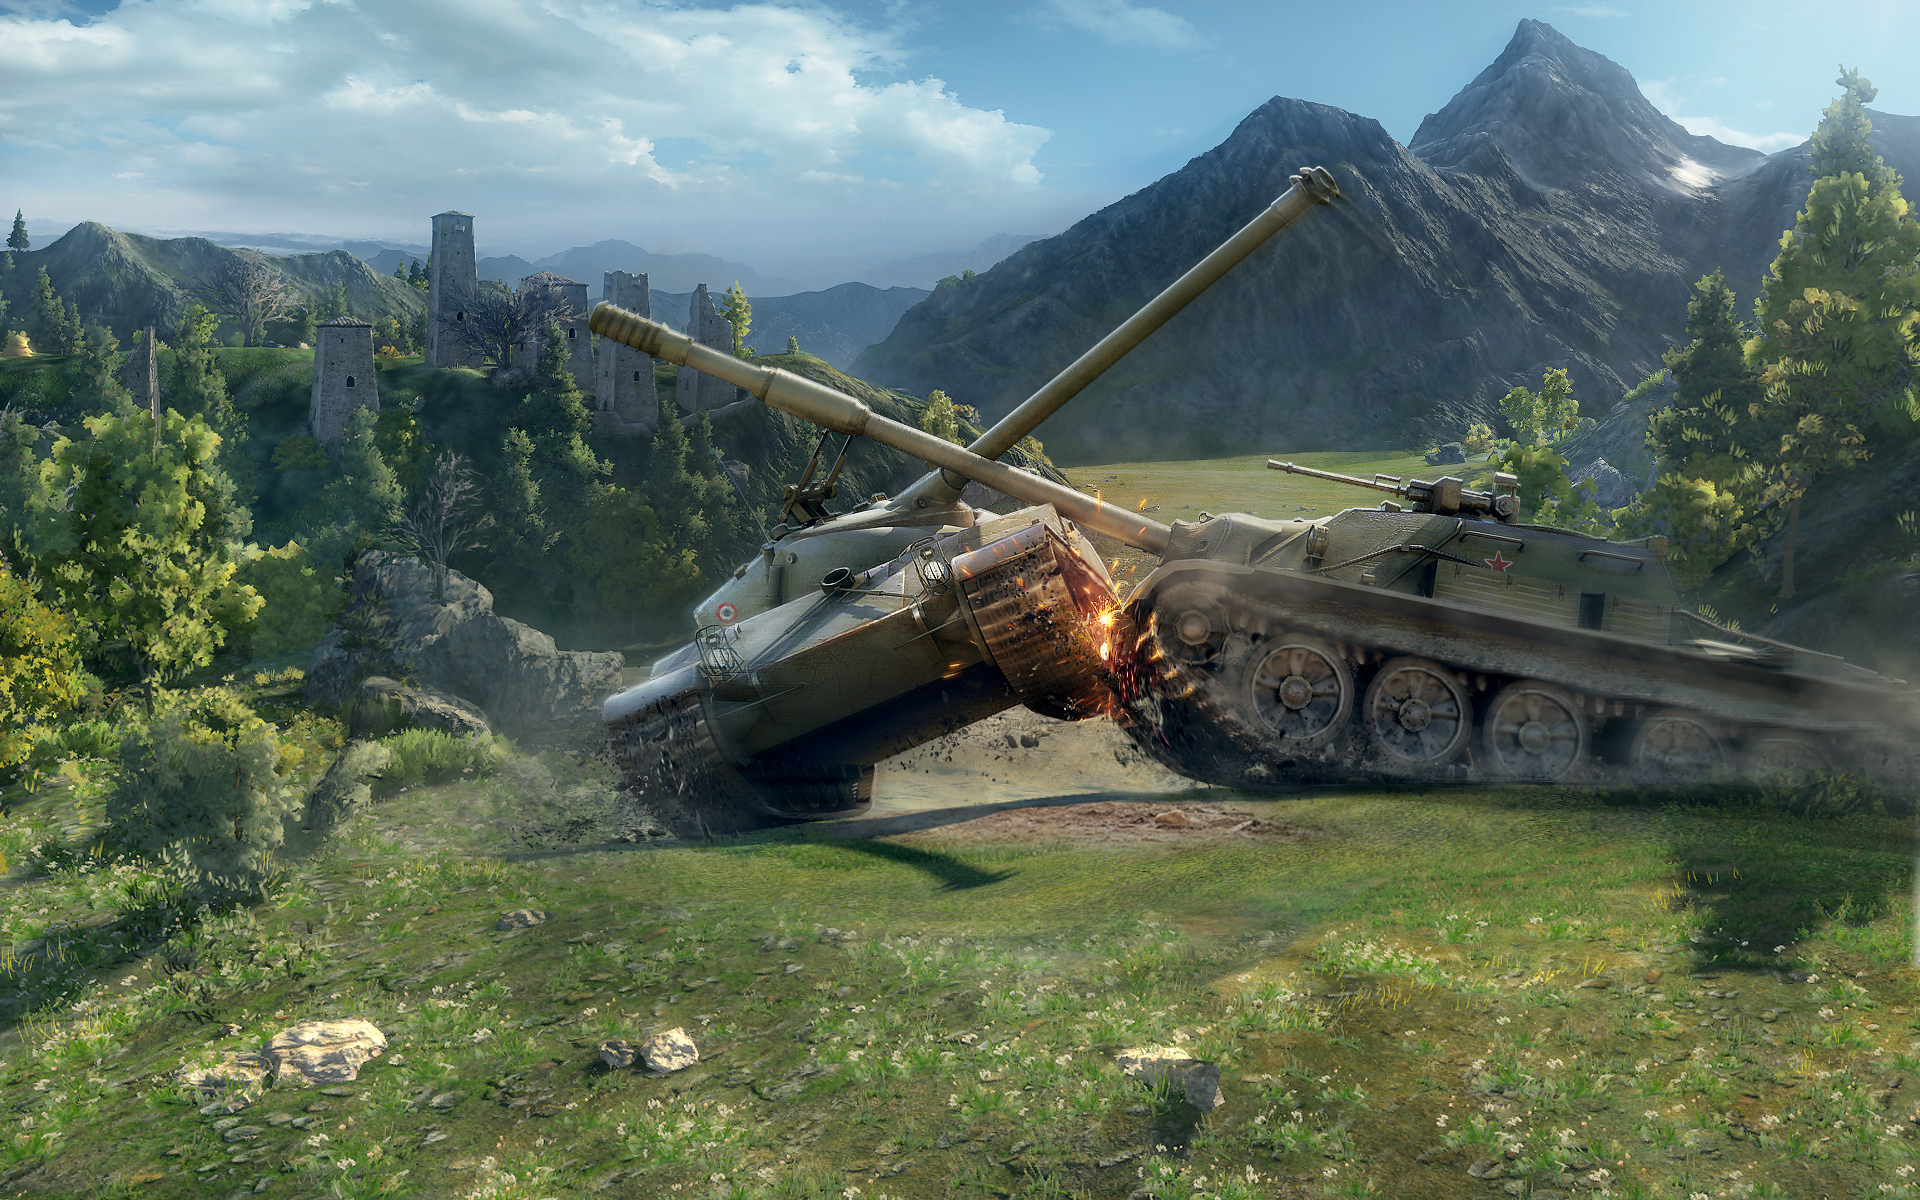
\includegraphics[width=\paperwidth]{wot.jpg}}
\begin{frame}[plain]{}
\end{frame}
}

\begin{frame}{ПЛАТА ВПЕРЁД}
    \begin{enumerate}
        \item LVEE
        \item Linux Foundation
        \item Django Foundation
        \item Python Software Foundation
        \item Wikimedia Foundation
        \item Python Meetup в Минске
    \end{enumerate}
\end{frame}

\begin{frame}{ИДЕИ}
    \begin{itemize}
        \item Linux на сервере --- ключ к успеху
        \item опора на Open Source --- второй ключ к успеху
        \item главное --- скорость и простота разработки
        \item не стоит бояться гетерогенной среды
        \item полный контроль над всеми частями системы
    \end{itemize}
\end{frame}

{
\setbeamertemplate{footline}{}
\setbeamercolor{frametitle}{fg=white}
\setbeamercolor{normal text}{fg=white}
\setbeamercolor{block title}{fg=white}
\setbeamercolor{block body}{fg=red}

\usebackgroundtemplate{
\includegraphics[height=\paperheight]{wg-end.jpg}}
\begin{frame}{СПАСИБО ЗА ВНИМАНИЕ. ВОПРОСЫ}
    \begin{block}{Максим Мельников}
    \par \url{mailto:m\_melnikau@wargaming.net}
    \par \url{https://plus.google.com/114669104565190507739/}
    \par \url{https://twitter.com/max\_posedon}
    \par \url{http://wargaming.com}
    \end{block}
\end{frame}
}

\end{document}
